\section{Decentralised Exchange using Lightning Network} \label{sec:dex}

Via a TSN, interfacing other alien \abbrev{DLT}{Distributed Ledger Technology} for exchanges is possible. Most of the current DLTs are based on \abbrev{POW}{Prof Of Work} which secures the immutability of the ledger and has been proven to be very robust. The downside for those types of DLT is the long confirmation time.\\
A suggested solution to decreasing the confirmation time is to use a second layer solution using a network of payment channels like the \abbrev{LN}{Lightning Network}.\\
\abbrev{TN}{Tagion Network} and LN support each other to enable a \abbrev{DEX}{Decentralised Exchange} for DLT networks which support full-duplex payment channels, \abbrev{HTLC}{Hashed Time Lock Contract} and \abbrev{MultSig}{Multi Signature}.
The advantage of using the TN as a support system to store intermediate data for the payment channels is that the LN-nodes can share data even if some of the LN nodes go offline.
In the current LN use in Bitcoin and other similar networks, the routing between the payment channels is a challenge. One of the reasons for this is that the routing tables are difficult to share and maintain between the nodes. In Tagion, because data is stored in a DART this makes sharing data feasible.\\
Because funds in an alien DLT can be locked via an HTLC, the \abbrev{ALC}{alien-currency} the funds can be swapped with the native tagion-currency in an atomic manner. This feature enables the Tagion network to support exchange functionality in a decentralised manner providing full liquidity because all exchange pairs have Tagions as the counterpart.\\

\subsection{Trading flow using Lightning and Tagion Network}
The Tagion network can order the bids/asks in a \abbrev{BFT}{Byzantine Fault Tolerant} manner. This means that the network is able to come to a consensus on the order of transactions and this solves the matching and prices discovery in a fair manner and solves front-running the order-book in a decentralised manner.

The idea is one STN handles only one trading pair between TGS and ALC. By only using one pair, the matching and routing problem is reduced significantly in comparison to a full multi-currency-DEX with more than two currencies.\\
First of all, the price discovery is more straightforward, and the amount of data to process is much less if only one pair must be matched and discovered. The second advantage of the one pair DEX is that sub-networks only need to handle one alien smart contract format.\\

\subsubsection{Price discovery and matching}

The DEX are able to handle two types of orders as shown in \cref{tab:dex_acl_tgn} and \cref{tab:dex_tgn_acl}.
The orders are sent to the TN and at each epoch the trade-order-queue is sorted according to the hashgraph consensus ordering. 
\paragraph{Exchange order pairs}
\begin{itemize}
 \item[\bfit{ATO}] Order to buy TGS for ALC
 \item[\bfit{BTO}] Order to buy ALC for TGS
\end{itemize}

The matching-engine will maintain two sales-lists of \abbrev{ATO}{Ask Trade Orders} and a \abbrev{BTO}{Bid Trade Orders}, those sales-lists are sorted according to the exchange rate with the lowest exchange ratio at to top of the list. A detailed example can be found in \cref{sec:dex_example}.


The \bfit{ask} exchange rate is defined as:
\begin{equation}
 E_{ask} = \frac{Q}{P} ~\text{in unit} ~\left[ ACL/TGS \right]
\end{equation}

The \bfit{bid} exchange rate is defined as:
\begin{equation}
 E_{bid} = \frac{P}{Q}~\text{in unit} ~\left[ TGS/ACL \right]
\end{equation}

\begin{itemize}
 \item[$P$]is the price in TGS
 \item[$Q$]is the price in ACL
\end{itemize}


The trade-order-queue is maintained with the orders that are not executed. A new trade-order-queue is generated in each epoch and added in the end of the current trade-order-queue.
The matching executes the first in trade-order-queue, i.e. the oldest order is searched first for a match.

The ATO and BTO order in the trade-order-queue are defined as buyers.
A match is defined as found, when the buyer's exchange-rate is higher than or equal to the seller's exchange-rate from the corresponding sales-list. The price of the settlement will be set at the seller's exchange-rate.
\begin{itemize}
 \item 
When an ATO buys from BTO-sales-list at $E_{ask,BTO}$ price when:\\ $E_{ask,ATO} \geq E_{ask,BTO}$ or the same as $\frac{Q_{ATO}}{P_{ATO}} \geq \frac{Q_{BTO}}{P_{BTO}}$.
 \item 
When an BTO buys from ATO-sales-list at $E_{bid,ATO}$ price when:\\ $E_{bid,BTO} \geq E_{bid,ATO}$ or the same as $\frac{P_{BTO}}{Q_{BTO}} \geq \frac{P_{ATO}}{Q_{ATO}}$.
\end{itemize}

Summarising, a buyer with an ATO-order from the order-queue matches a seller with a BTO-order from the BTO-sales-list and vice versa. 
Then the size is calculated, and a trading-contract with the corresponding pair is generated and stored in the TN.

If the ATO or the BTO has sold the whole size, then the order is removed from the lists.\\
If an order includes a valid time period of $t$ and if the epoch consensus time is greater than this valid time period $t$ then the order is removed and not executed.

\begin{table}[H]
\begin{center}
\begin{tabular}{|l|p{7cm}|p{1.5cm}|l|}
      \hline
      Parameter & Description &  Type & Access \\
      \hline
      $\$type$ & Set the contract type to 'ATO' &  \texttt{string} & \texttt{ro}\\
      \hline
      $P$ & Price unit TGS &  \texttt{ulong} & \texttt{ro}\\
      \hline
      $Q$ & Price unit ACL &  \texttt{ulong} & \texttt{ro} \\
      \hline
      $size$ & Size of ACL &  \texttt{ulong} & \texttt{ro}\\
      \hline
      $lock$ & Random Hash-lock key &  \texttt{bin} & \texttt{ro}\\
      \hline
      $time$ & Valid time period &  \texttt{utc} & \texttt{ro} \\
      \hline
  \end{tabular}
\end{center}
\caption{ATO HiBON to buy TGS for ALC} 
\label{tab:dex_tgn_acl}
\end{table}

\begin{table}[H]
\begin{center}
\begin{tabular}{|l|p{7cm}|p{1.5cm}|l|}
      \hline
      Parameter & Description & Unit & Access \\
      \hline
      $\$type$ & Sets the contract type to 'BTO' &  \texttt{string} & \texttt{ro}\\
      \hline
      $P$ & Price unit TGS &  \texttt{ulong}& \texttt{ro}\\
      \hline
      $Q$ & Price unit ACL &  \texttt{ulong}& \texttt{ro} \\
      \hline
      $size$ & Size og TGS & \texttt{ulong}& \texttt{ro} \\
      \hline
      $lock$ & Random Hash-lock key & \texttt{bin} & \texttt{ro} \\
      \hline
      $time$ & Valid time period & \texttt{utc} & \texttt{ro} \\
      \hline
  \end{tabular}
\end{center}
\caption{BTO HiBON to buy ALC for TGS} 
\label{tab:dex_acl_tgn}
\end{table}


\subsubsection{Exchange execution rules}
\begin{figure}[H]
 \centering
 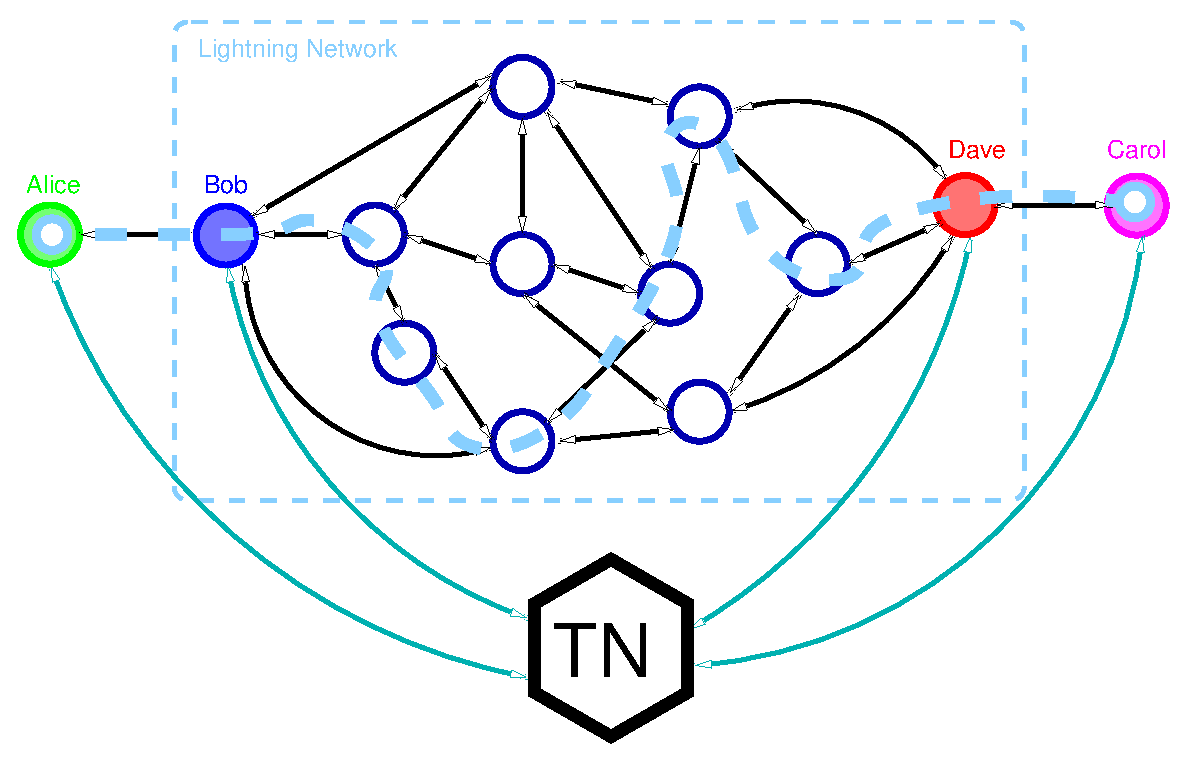
\includegraphics[width=1.0\textwidth]{fig/dex_ln.eps}
 % dart_bw.eps: 17766x12625 px, 300dpi, 150.42x106.89 cm, bb=0 0 4264 3030
 \caption{Tagion Decentralised Exchange based on Lightning Network  }
 \label{fig:dex_ln}
\end{figure}

In the following example, the execution flow of the DEX is described.


\paragraph{Alice wants to trade TGS for ALC (ATO). It can be done as follows.}

\begin{enumerate}[{A}.1]
 \item \textbf{Entry:} Alice opens an LN channel with Bob.
 \item Alice requests a trading channel from Bob with a guarantee of $\omega_{alice,S}$ in ALC 
 \item Bob locks up a guarantee of an amount $\tau_{bob,S}$ in TGS which matching Alice's $\omega_{alice,S}$ amount. Bob creates an HTLC lock it with $R_{bob}$ and send this information to the TN.
 \item Alice pays $\omega_{alice}$ to the contract lock with $R_{bob}$.
 \item \textbf{Order:} Alice sends an order to the TN including an HTLC contract to Bob locked with $R_{alice}$ and the amount $\alpha_{alice}$ in ALC. The information includes the bid/ask prices and HTLC contract which is sent to the TN.\\
 \textit{\textbf{Note:} Carol has previously locked funds with $R_{calor}$ in TGS to buy ALC}
 \item When the TN discoveries a trading pair matching Alice and Carol the network generated a TN-HTLC trading contract locked with both $R_{alice}$ and $R_{carol}$.
 \item When Bob verifies that, Carol has to reveal $R_{calor}$. Bob initials a route between Alice to Carol according to the trading bill. Bob also makes an HTLC return the rest of Alice's funds locked with $R_{alice}$.
 \item Alice reveals $R_{alice}$ and the funds can be transferred.
 \item \textbf{Exit:} Alice can ask Bob to reveal $R_{bob}$ and exit the trading channel. Bob's locked funds are returned, and Alice can claim her funds.  
\end{enumerate}

\paragraph{Carol wants to trade ALC for TGS (BTO). It can be done as follows}
\begin{enumerate}[{B}.1]
 \item \textbf{Entry:} Carol opens an LN channel with Dave.
 \item Carol requests a trade channel with Dave, both Carol and Dave guarantee $\tau_{carol,S}$ and $\tau_{dave,S}$ in TGS and hash-locked with $R_{carol}$ in the TN.
 \item \textbf{Order:} Carol sends an order to Dave via the TN.
 \item Dave receives a confirmation from the network about the order from Carol.  
 \item Dave and creates an HTLC contract to Carol locked with $R_{dave}$ at the amount of $\alpha_{carol,T}$ in ALC.
 \item When the TN discovers a trading pair matching Alice and Carol, the network generates a TN-HTLC trading contract locked with both $R_{alice}$ and $R_{carol}$.
 \item Dave reveals the $R_{dave}$ the Alice can execute the trade.
 \item \textbf{Exit:} Carol can ask Dave to reveal $R_{dave}$ and exit the trading channel. Dave's and Carol's locked funds are returned.  
 
\end{enumerate}

\begin{figure}[H]
 \centering
 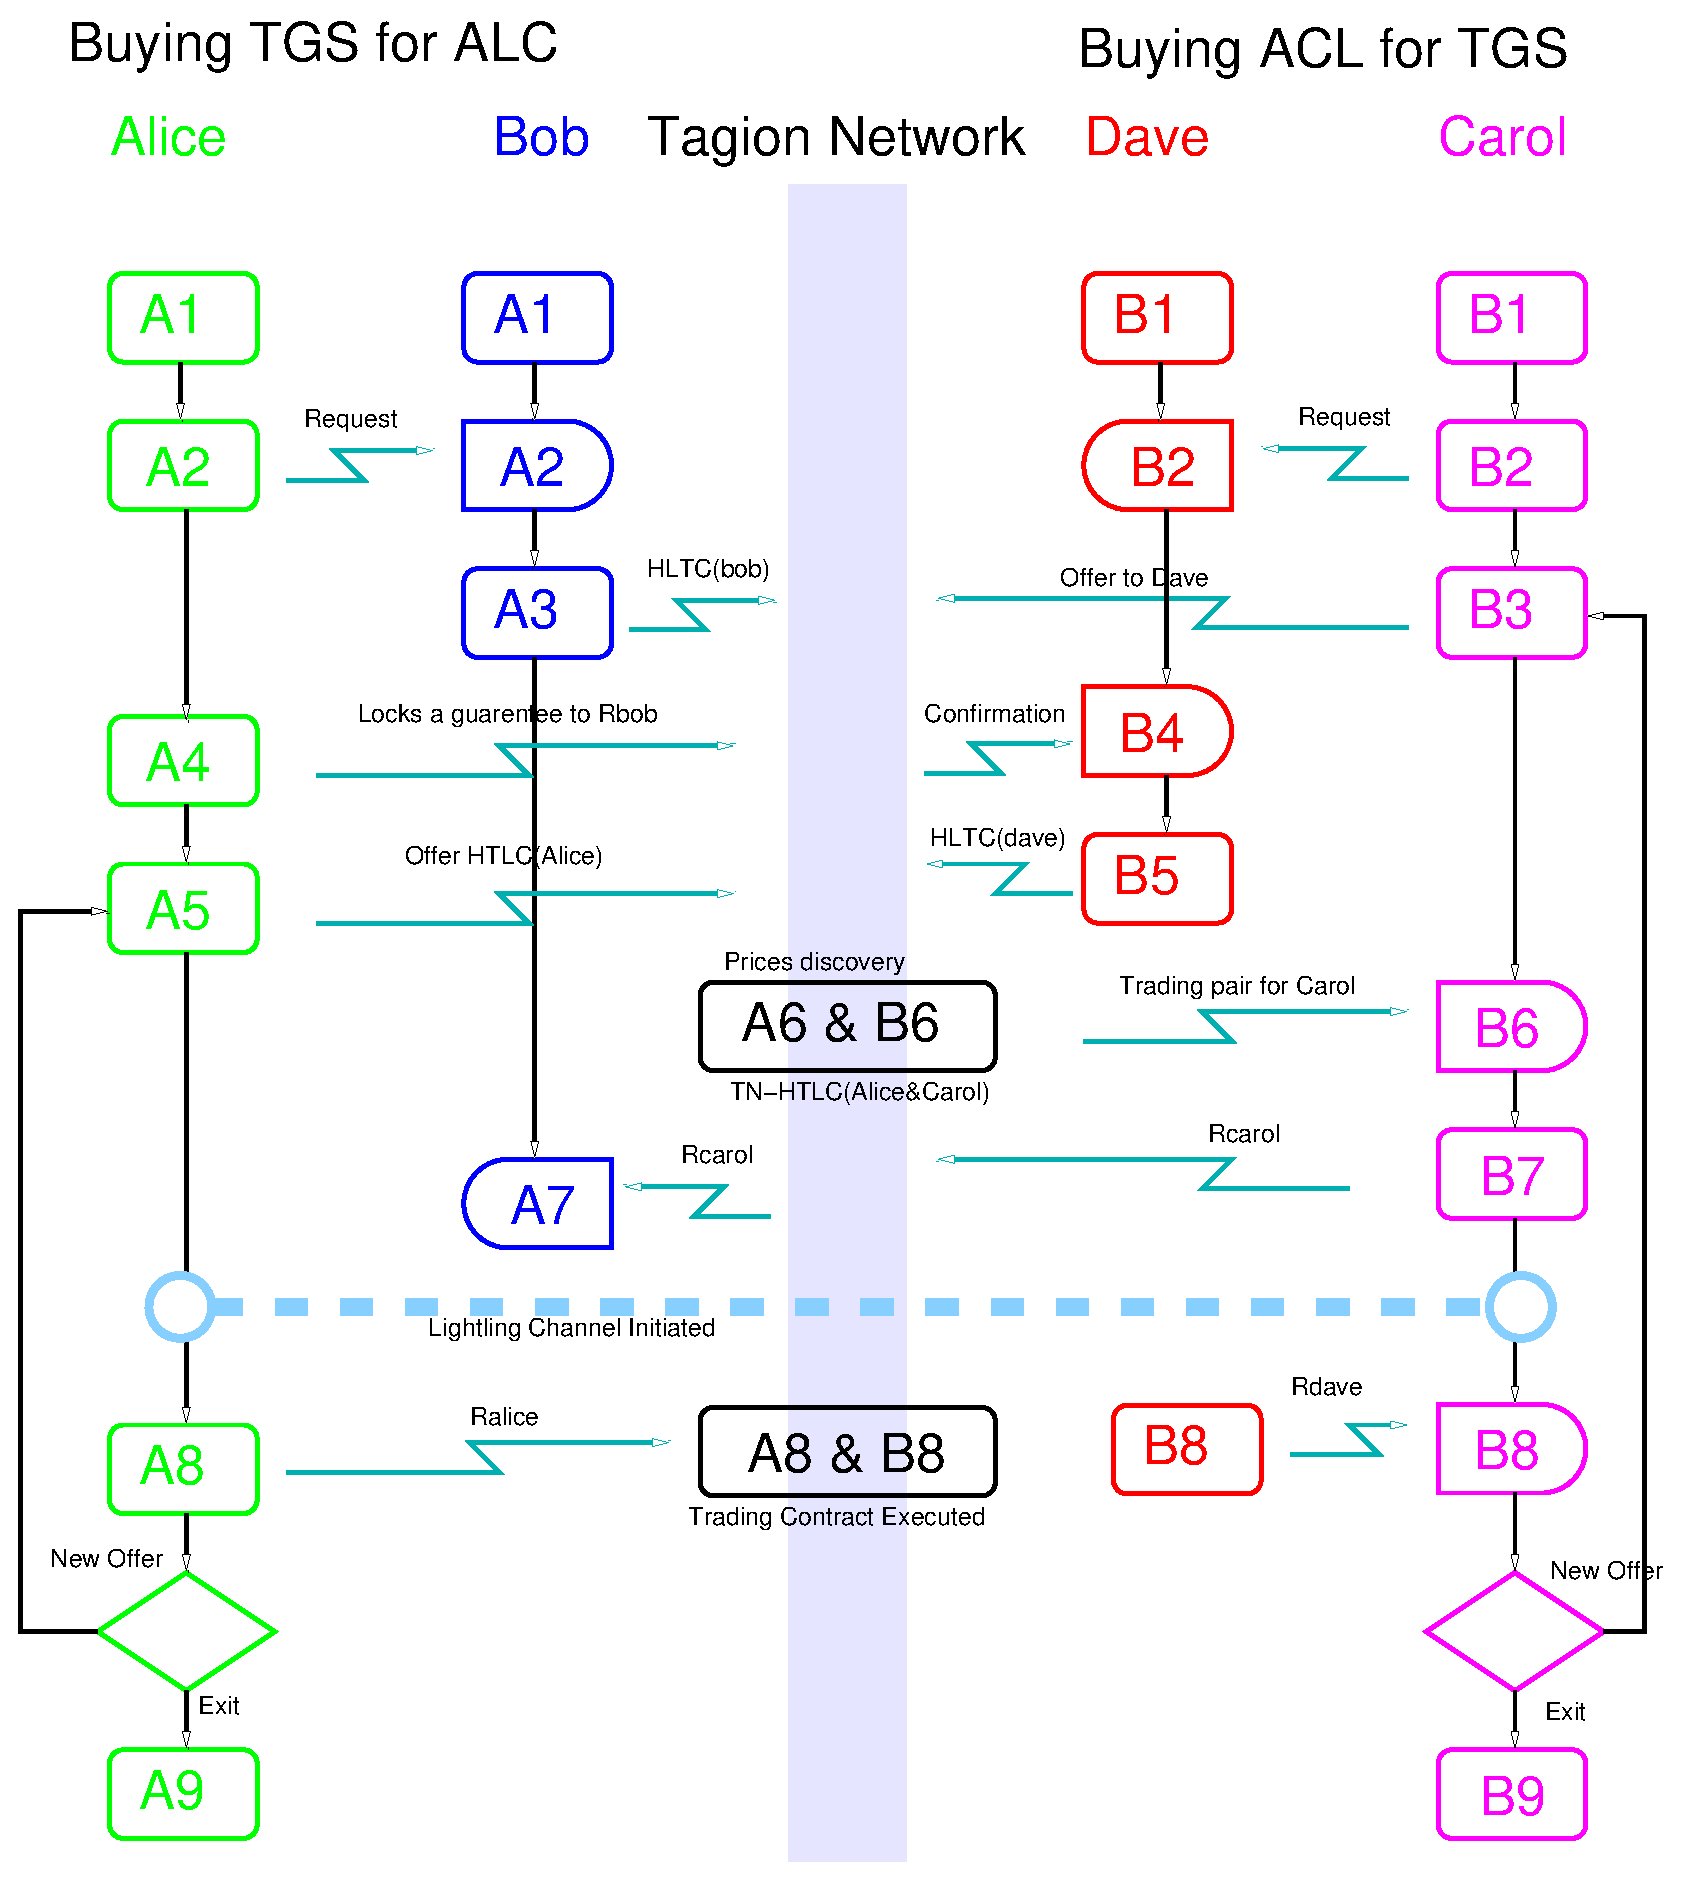
\includegraphics[width=1.0\textwidth]{fig/dex_flow.eps}
 \caption{DEX transaction flow}
 \label{fig:dex_flow}
\end{figure}

\paragraph{Incentives and Penalty}
If one or more of the 4 participants (Alice, Bob, Carol and Dave) fails to execute the trade, the flowing penalty rules will be performed by the TN consensus.
%\begin{enumerate}
\begin{enumerate}[\S 1]
\item \textbf{Alice doesn't claim the transaction} 
 \begin{description}
  \item \textbf{Incident} 
   \begin{itemize}
    \item 
    If Alice does not reveal $R_{alice}$ within the timeout limit.
   \end{itemize}
    \item \textbf{Action}
  \begin{itemize}
    \item 
    After a timeout period less than the Alice HLTC time lock.
    \item 
    The funds will be reverted to Carol.
    \item 
    The trade is deleted.
    \item 
    Bob keeps Alice's stacked fund's.
    \item 
    If the price of Alice's funds is less than Bob's guaranteed funds, Bob gets some of his funds back, which corresponds to the current trading prices.
    \item 
    The rest of Bob funds is burned.
    \item 
    If Alice reveals the $R_{alice}$ after the timeout, Alice loses her funds to Carol.
  \end{itemize}
 \end{description}
    \item \textbf{Bob doesn't initial the routing}
 \begin{description}
  \item \textbf{Incident}
   \begin{itemize}
    \item 
  If Bob is offline or choses not establish a connection within the a timeout period.
   \end{itemize}
  \item \textbf{Action}
   \begin{itemize}
    \item 
    Bob loses his funds and the trade bill is deleted.
    \item 
    Carol's funds are returned.
    \item 
    Alice will get her funds back after the HTLC time lock runs out.
   \end{itemize}
 \end{description}
 \item \textbf{Carol doesn't claim the transaction}
 \begin{description}
   \item \textbf{Incident} 
   \begin{itemize}
    \item 
    Carol does not reveal the $R_{carol}$ within the timeout limit.
   \end{itemize}
   \item \textbf{Action}
   \begin{itemize}
    \item 
    If Bob makes creates a contract which returns Alice's funds with a time limit Bob gets his funds back.
   \item
    Carol's transaction stake is burned and the rest of the funds is returned to Carol.
   \item
    The transactions bill is deleted.
   \end{itemize}
 \end{description} 
 \item \textbf{Dave doesn't accept the routing}
 \begin{description}
   \item \textbf{Incident} 
   \begin{itemize}
    \item 
    If Dave is offline or choses not establish connection within the a timeout period.
   \end{itemize}
   \item \textbf{Action}
   \begin{itemize}
    \item 
    After the timeout Carol can reclaim the stack $\omega_{carol}$ and open a new channel with Eric.
    \item
    Dave's stack $\omega_{dave}$ is burned
    \item
    Carol can initial the trade by revealing $R_{carol}$.
   \item
    The transaction's bill is deleted after execution.
   \end{itemize}
 \end{description} 
\end{enumerate}
